\documentclass[a4paper,12pt]{report}

% --- CẤU HÌNH TIẾNG VIỆT & FONT ---
\usepackage[utf8]{inputenc}
\usepackage[T5]{fontenc} % Bắt buộc cho tiếng Việt
\usepackage[vietnamese]{babel}
\usepackage{lmodern}
\usepackage{mathptmx} % Font giống Times New Roman, gọn gàng hơn cho báo cáo

% --- CÁC GÓI HỖ TRỢ ---
\usepackage{geometry}
\usepackage{amsmath, amssymb, amsfonts}
\usepackage{graphicx}
\graphicspath{{../figures/}}
\usepackage{svg} % Hỗ trợ file SVG
\usepackage{booktabs}
\usepackage{float}
\usepackage{enumitem}
\usepackage{cite}
\usepackage[hyphens]{url} % Hỗ trợ URL trong bibliography với khả năng xuống hàng
\usepackage{xcolor}
\usepackage{titlesec}
\usepackage{caption}
\usepackage[breaklinks=true,hidelinks]{hyperref} % Cho phép URL xuống hàng

% --- CẤU HÌNH URL ---
\def\UrlBreaks{\do\/\do\-\do\.\do\=\do\?\do\&} % Cho phép URL break tại các ký tự này
\urlstyle{same} % Giữ nguyên font như văn bản

% --- CẤU HÌNH TRANG ---
\geometry{left=2.5cm, right=2.5cm, top=2.5cm, bottom=2.5cm}
\linespread{1.2} % Giãn dòng 1.2 cho thoáng, dễ đọc
\setlength{\parskip}{6pt} % Khoảng cách giữa các đoạn văn

% Dùng section làm cấp cao nhất trong lớp report (tránh đánh số 0.x)
\renewcommand{\thesection}{\arabic{section}}

% Nạp các chỉ số thống kê được sinh tự động từ pipeline EDA
% dummy stats file
\newcommand{\digitTotal}{60000}
\newcommand{\digitCountZero}{5923}


\begin{document}

% --- TRANG BÌA ---
\begin{titlepage}
    \centering
    
    % Logo trường (Nếu bạn có file logo.png thì bỏ comment dòng dưới)
    % 
\includegraphics[width=0.25\textwidth]{logo.png} 
    \vspace{0.5cm}
    
    % Tên trường
    {\large \textbf{ĐẠI HỌC QUỐC GIA THÀNH PHỐ HỒ CHÍ MINH}}\\
    {\large \textbf{TRƯỜNG ĐẠI HỌC KHOA HỌC TỰ NHIÊN}}\\
    
    \vspace{0.3cm}
    \rule{0.6\textwidth}{0.5pt}
    \vspace{1cm}
    
    % Môn học
    {\Large \textbf{BÁO CÁO MÔN HỌC}}\\
    \vspace{0.3cm}
    {\LARGE \textbf{THỊ GIÁC MÁY TÍNH}}
    
    \vspace{2cm}

    
\begin{figure}[H]
    \centering
    % Đảm bảo bạn có file architecture.png trong thư mục dự án
    
\includegraphics[width=0.3\linewidth]{logo.png} 
\end{figure}
    
    
    % Đề tài
    \begin{minipage}{0.9\textwidth}
        \centering
        {\LARGE \textbf{PHÂN TÍCH THỐNG KÊ CÁC TẬP DỮ LIỆU MNIST}}
    \end{minipage}

    \vfill

    \vspace{1cm}
    
    \begin{minipage}{\textwidth}
        \centering
        {\large \textbf{Giảng viên hướng dẫn:}}
        \vspace{0.3cm}
        {\large {TS. Võ Hoài Việt}}
    \end{minipage}
    
    % Thông tin sinh viên và giảng viên
    \begin{minipage}{\textwidth}
        \centering
        {\large \textbf{Sinh viên thực hiện:}}\\
        \vspace{0.3cm}
        {Lê Anh Duy (23127011)}
    \end{minipage}
    
    \vspace{1.5cm}
    
    % Thời gian
    {\large Thành phố Hồ Chí Minh, \today}
    
\end{titlepage}

% --- MỤC LỤC ---
\newpage
\tableofcontents
\newpage

\section{Khởi tạo \& Tiền xử lý}
\subsection{Mục tiêu}
Thiết lập pipeline tải dữ liệu đồng nhất cho ba bộ MNIST (Digit, Fashion, Pneumonia), chuẩn hóa dữ liệu về cùng định dạng số học, và trình bày thống kê cơ bản để bảo đảm tính so sánh công bằng giữa các tập dữ liệu.

\subsection{Thao tác}
Sử dụng \texttt{tensorflow.keras.datasets} để tải Digit MNIST và Fashion MNIST, và sử dụng thư viện \texttt{medmnist} để tải trực tiếp tập PneumoniaMNIST (bộ X-quang ngực thuộc MedMNIST v2).\footnote{\url{https://medmnist.com/}} Kích thước ảnh gốc của cả ba bộ dữ liệu là 28\,$\times$\,28 (grayscale) - giá trị điểm ảnh trong khoản [0, 255]; chuẩn hóa giá trị điểm ảnh về dải $[0,1]$ bằng cách chia cho 255. Sau khi tải, tập huấn luyện và tập kiểm tra của mỗi bộ dữ liệu được gộp chung lại với nhau nhằm có cái nhìn toàn diện khi EDA. Notebook EDA đầy đủ: \url{https://github.com/Le-Anh-Duy/CV-HOMEWORK-2-Mnist-EDA/blob/main/notebooks/download_data_eda.ipynb}.

\subsection{Thông tin ban đầu của dữ liệu}
Bảng \ref{tab:raw-dataset-summary} tóm tắt các thông số gốc trước khi chuẩn hóa (kích thước ảnh, số lượng mẫu, số lượng lớp và miền giá trị điểm ảnh). Các giá trị điểm ảnh ban đầu nằm trong dải $[0,255]$ và được chuẩn hóa về $[0,1]$ ở bước tiền xử lý.

\begin{table}[H]
    \centering
    \caption{Tổng quan thông số gốc của các tập dữ liệu (trước chuẩn hóa)}
    \label{tab:raw-dataset-summary}
    \begin{tabular}{lrrrrl}
        \toprule
        \textbf{Dataset} & \textbf{Train} & \textbf{Test} & \textbf{Classes} & \textbf{Size} & \textbf{Value range} \\
        \midrule
        Digit MNIST & 60000 & 10000 & 10 & 28$\times$28 & [0,255] \\
        Fashion MNIST & 60000 & 10000 & 10 & 28$\times$28 & [0,255] \\
        PneumoniaMNIST & 4708 & 624 & 2 & 28$\times$28 & [0,255] \\
        \bottomrule
    \end{tabular}
\end{table}

\subsection{Insight}
Các tập dữ liệu có kích thước ảnh đồng nhất, nhưng số lượng mẫu và số lượng lớp khác nhau.

\section{Khảo sát Phân phối Nhãn}
\subsection{Mục tiêu}
Đánh giá độ cân bằng lớp của ba tập dữ liệu và xác định mức độ mất cân bằng nghiêm trọng ở PneumoniaMNIST.

\subsection{Thao tác}
Đếm số lượng mẫu mỗi lớp và vẽ biểu đồ cột cho từng tập trên cùng một hình (1 hàng, 3 cột). 

\subsection{Insight}
Digit/Fashion MNIST gần như cân bằng hoàn toàn, trong khi PneumoniaMNIST thể hiện chênh lệch mạnh giữa hai lớp (Hình~\ref{fig:label-distribution}). Tỷ lệ mất cân bằng cần được lưu ý để cân nhắc kỹ thuật \textit{class weighting} hoặc \textit{resampling} trong các mô hình sau.

\begin{figure}[H]
    \centering
    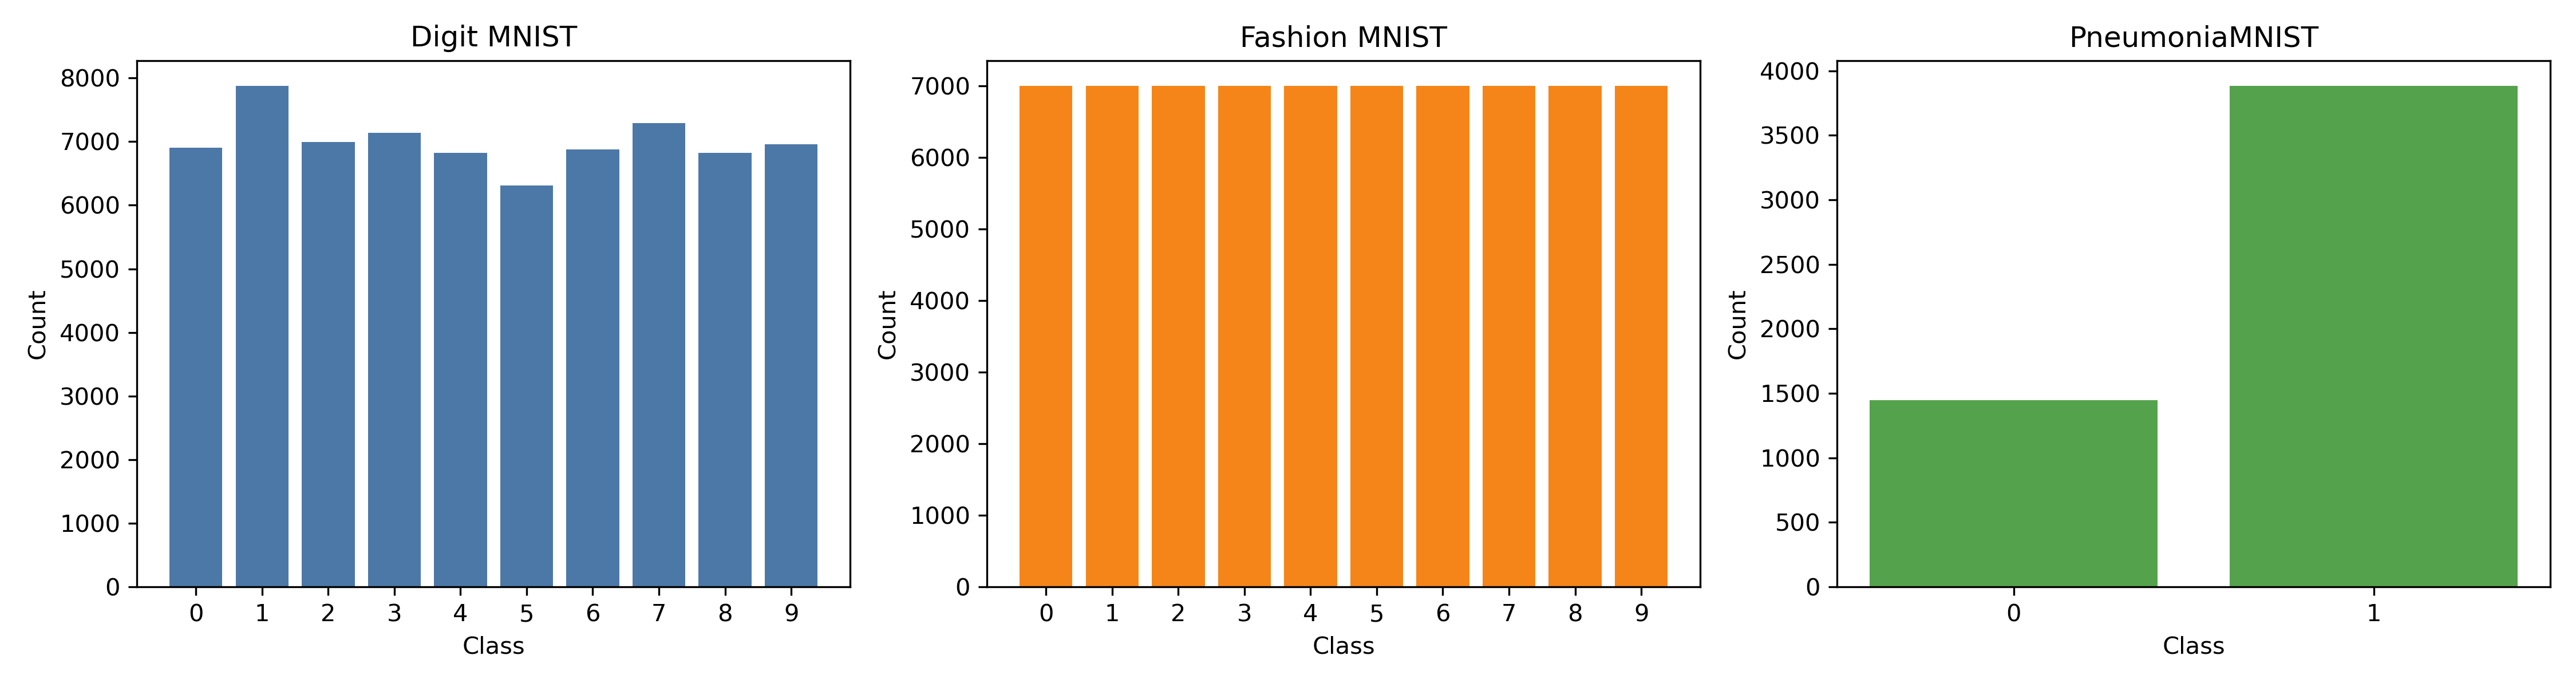
\includegraphics[width=0.9\linewidth]{label_distribution.png}
    \caption{Phân phối nhãn của Digit MNIST, Fashion MNIST và PneumoniaMNIST.}
    \label{fig:label-distribution}
\end{figure}

\section{Phân tích Phân phối Điểm ảnh}
\subsection{Mục tiêu}
So sánh phân phối cường độ điểm ảnh giữa Digit MNIST và PneumoniaMNIST để đánh giá khả năng phân biệt dựa trên độ sáng.

\subsection{Thao tác}
Vẽ histogram cường độ điểm ảnh cho Digit MNIST, Fashion MNIST và histogram chồng cho PneumoniaMNIST (Normal vs Pneumonia) để quan sát phân phối sáng tối. Bổ sung một biểu đồ tròn riêng cho Digit MNIST nhằm thể hiện tỷ lệ điểm ảnh rơi vào hai đỉnh 0 và 1 so với các giá trị trung gian khác.

\subsection{Insight}
Ở tập Digit và Fashion thì đa phần pixel là nền (giá trị 0). Phân phối hai đỉnh trong Digit MNIST phản ánh hai miền điểm ảnh: nền tối (pixel gần 0) và nét chữ sáng (pixel gần 1) (Hình~\ref{fig:pixel-histogram} và Hình~\ref{fig:digit-pixel-pie}). Tập Fashion thì lại có các giá trị phân bố đều hơn ở các pixel lớn hơn 0 nhưng không phải là 1 cột rõ ràng như digit, thể hiện trong tập này các chủ thể thường được thể hiện như 1 khối thay vì các nét như tập digit (Hình~\ref{fig:pixel-histogram}). Với PneumoniaMNIST, phân phối thường gần dạng chuông và hai lớp chồng lấn nhiều, cho thấy độ sáng đơn thuần không đủ để phân loại bệnh lý (Hình~\ref{fig:pixel-histogram}).

\begin{figure}[H]
    \centering
    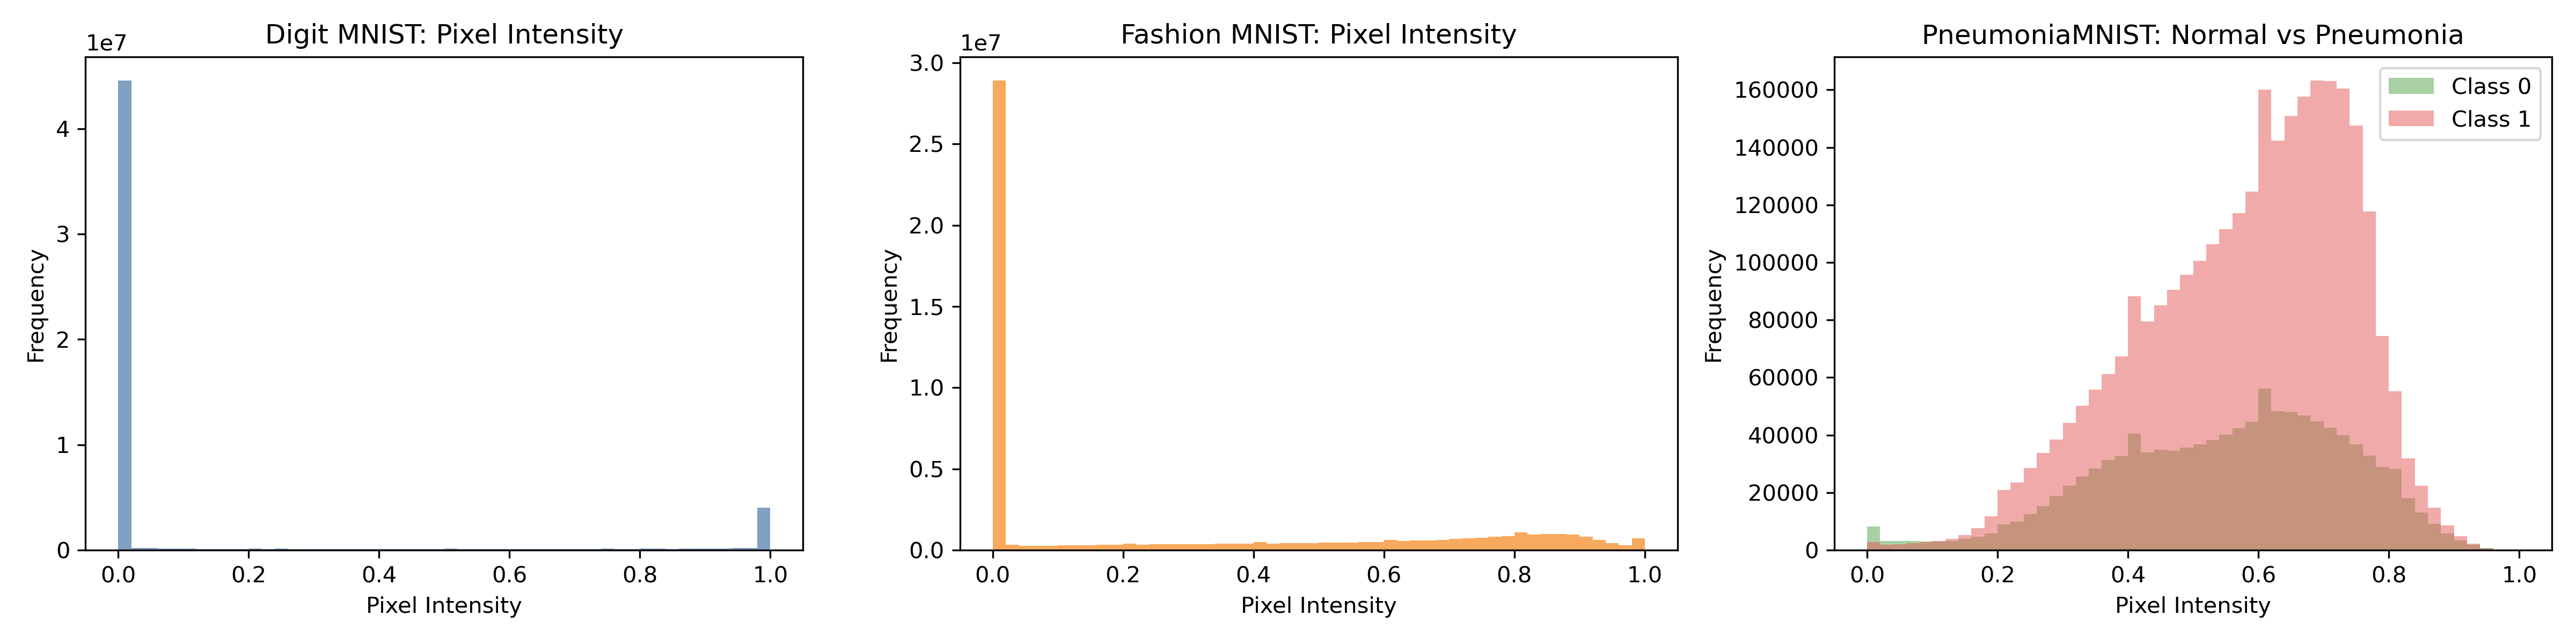
\includegraphics[width=0.95\linewidth]{pixel_histogram_digit_pneumonia.png}
    \caption{Histogram cường độ điểm ảnh: Digit MNIST, Fashion MNIST, và PneumoniaMNIST (Normal vs Pneumonia).}
    \label{fig:pixel-histogram}
\end{figure}

\begin{figure}[H]
    \centering
    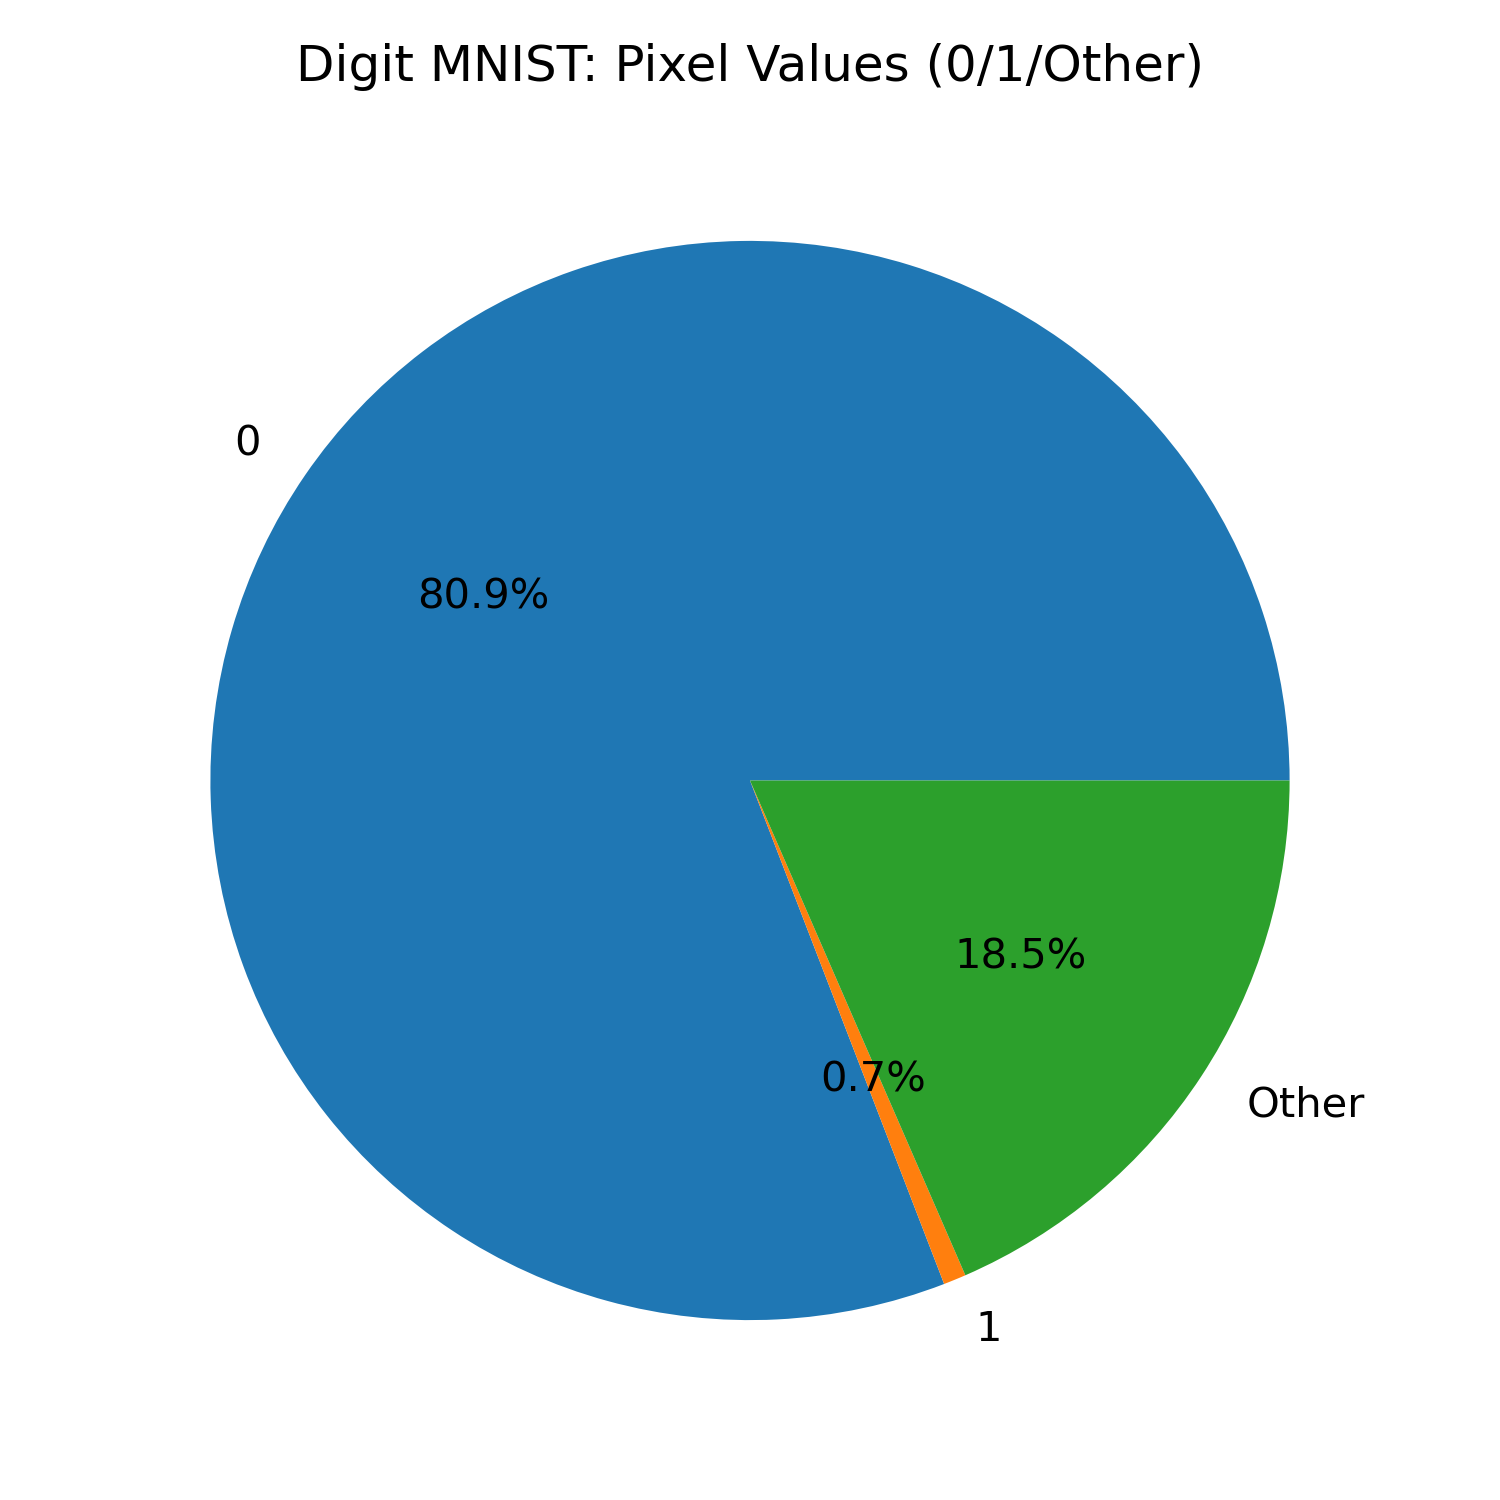
\includegraphics[width=0.55\linewidth]{digit_pixel_value_pie.png}
    \caption{Pie chart phân bố giá trị điểm ảnh của Digit MNIST (0/1/khác), nhấn mạnh hai đỉnh tại 0 và 1.}
    \label{fig:digit-pixel-pie}
\end{figure}

\section{Phân tích Ảnh Trung bình \& Bản đồ Chênh lệch}
\subsection{Mục tiêu}
Khám phá vùng tín hiệu chung của từng lớp thông qua ảnh trung bình, và định vị các vùng khác biệt không gian quan trọng ở PneumoniaMNIST.

\subsection{Thao tác}
Tính ảnh trung bình cho từng lớp của cả ba tập dữ liệu. Vẽ lưới ảnh trung bình (Digit: 2x5, Fashion: 2x5, Pneumonia: 1x2). Với PneumoniaMNIST, lấy ảnh trung bình của lớp Pneumonia trừ Normal, sau đó vẽ heatmap với bảng màu \texttt{RdBu\_r}.

\subsection{Insight}
Các ảnh trung bình của Digit/Fashion thể hiện rõ hình dáng đặc trưng theo lớp (Hình~\ref{fig:mean-digit} và Hình~\ref{fig:mean-fashion}). Ở PneumoniaMNIST, heatmap chênh lệch nhấn mạnh vùng phổi hai bên, trong khi vùng tim/giữa ngực có xu hướng trung tính, gợi ý vùng tín hiệu chính cho phân loại (Hình~\ref{fig:mean-pneumonia} và Hình~\ref{fig:pneumonia-diff}).

\begin{figure}[H]
    \centering
    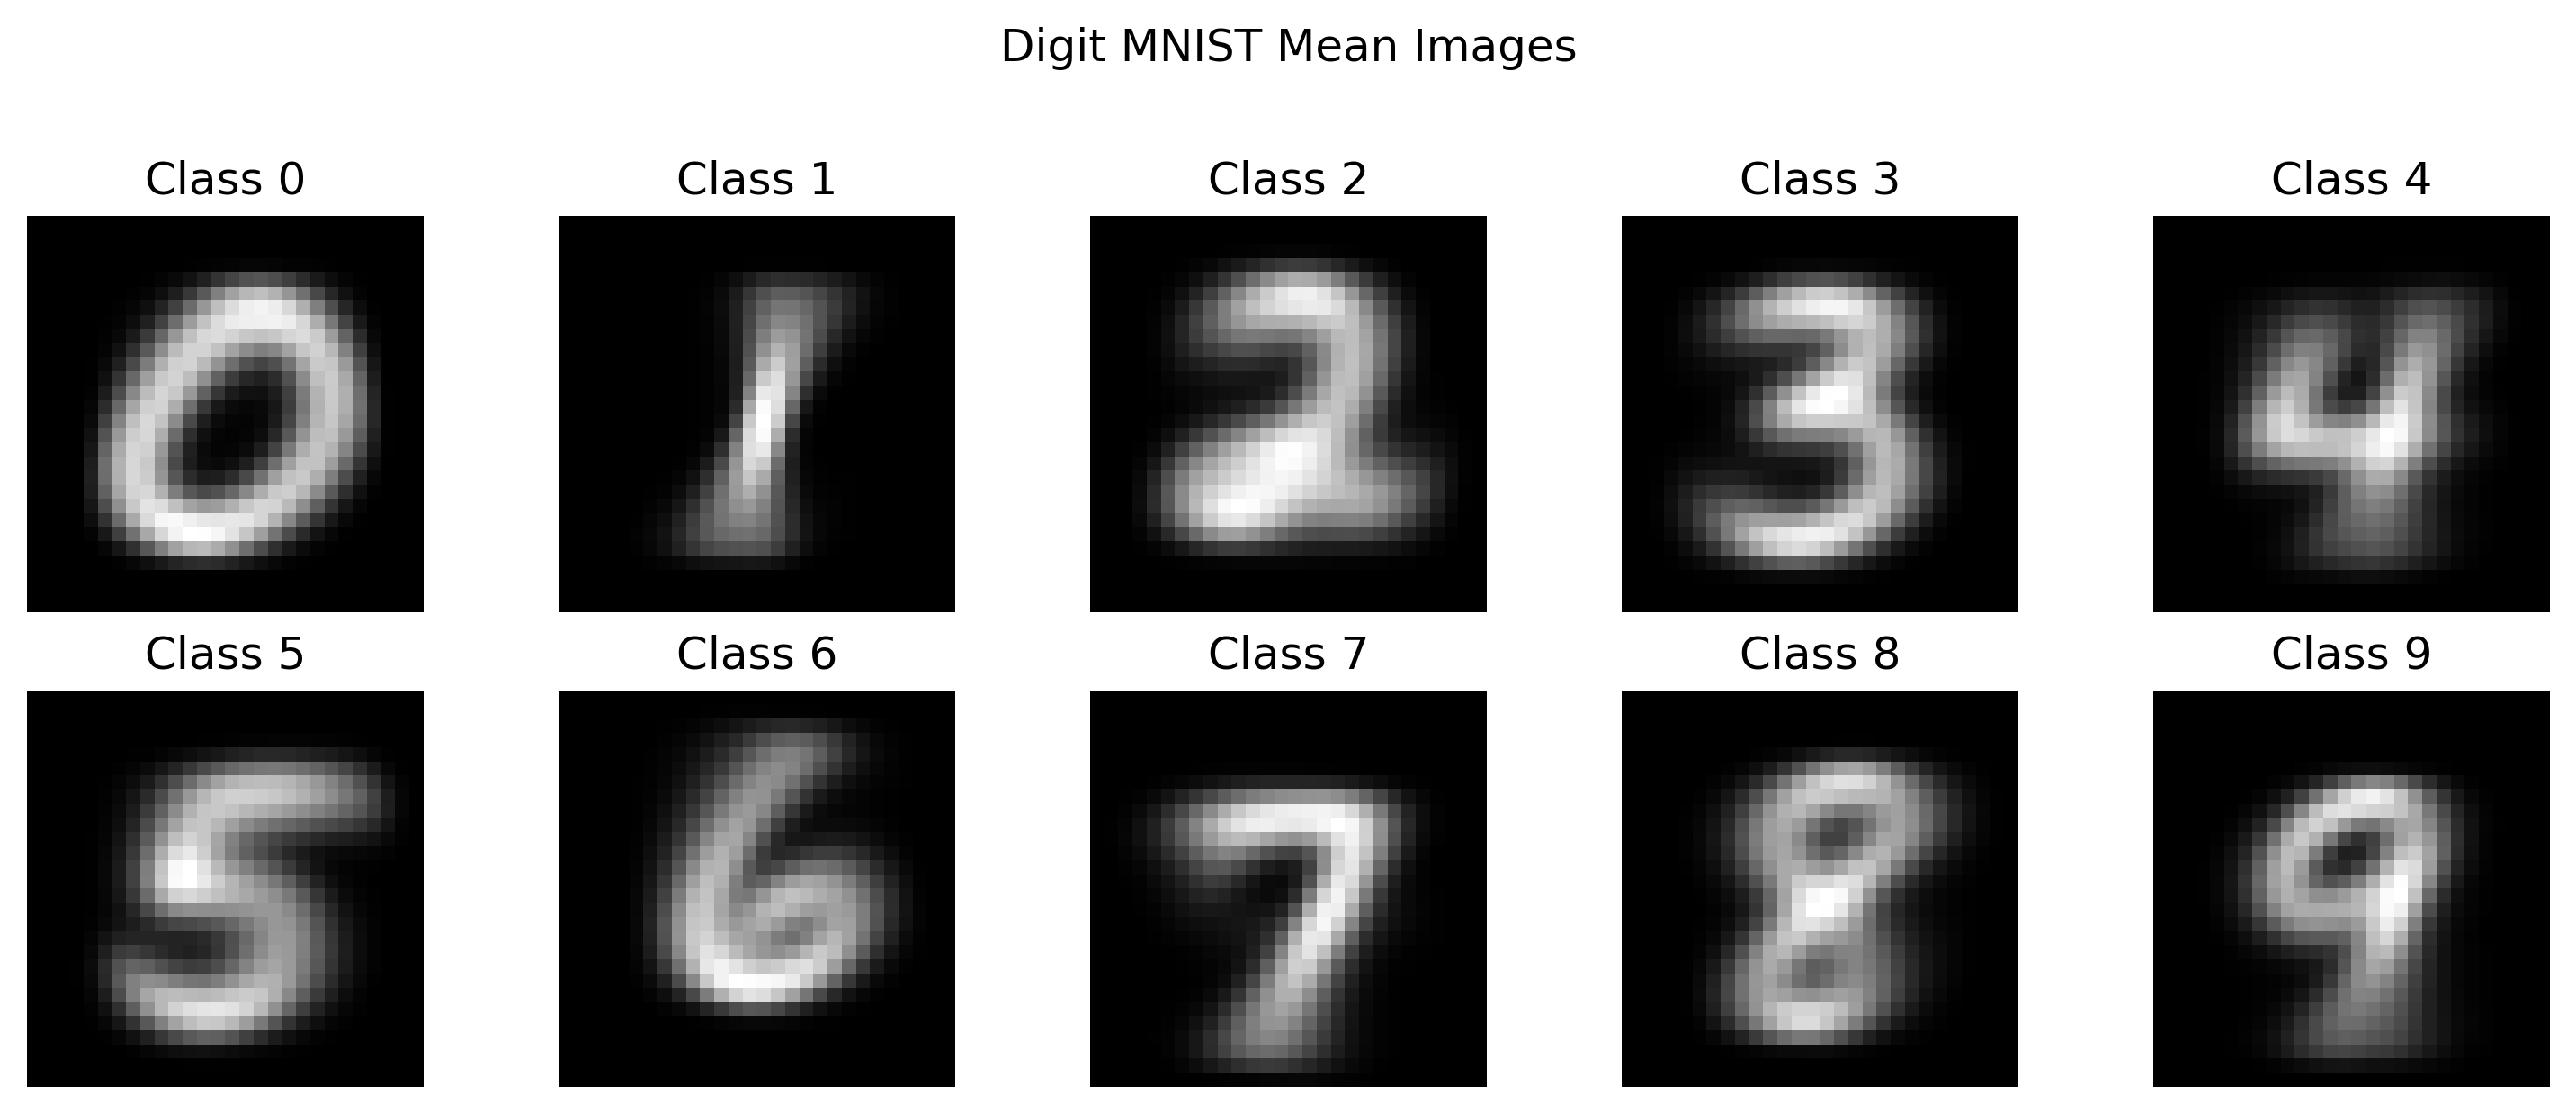
\includegraphics[width=0.9\linewidth]{mean_digit.png}
    \caption{Ảnh trung bình theo lớp của Digit MNIST.}
    \label{fig:mean-digit}
\end{figure}

\begin{figure}[H]
    \centering
    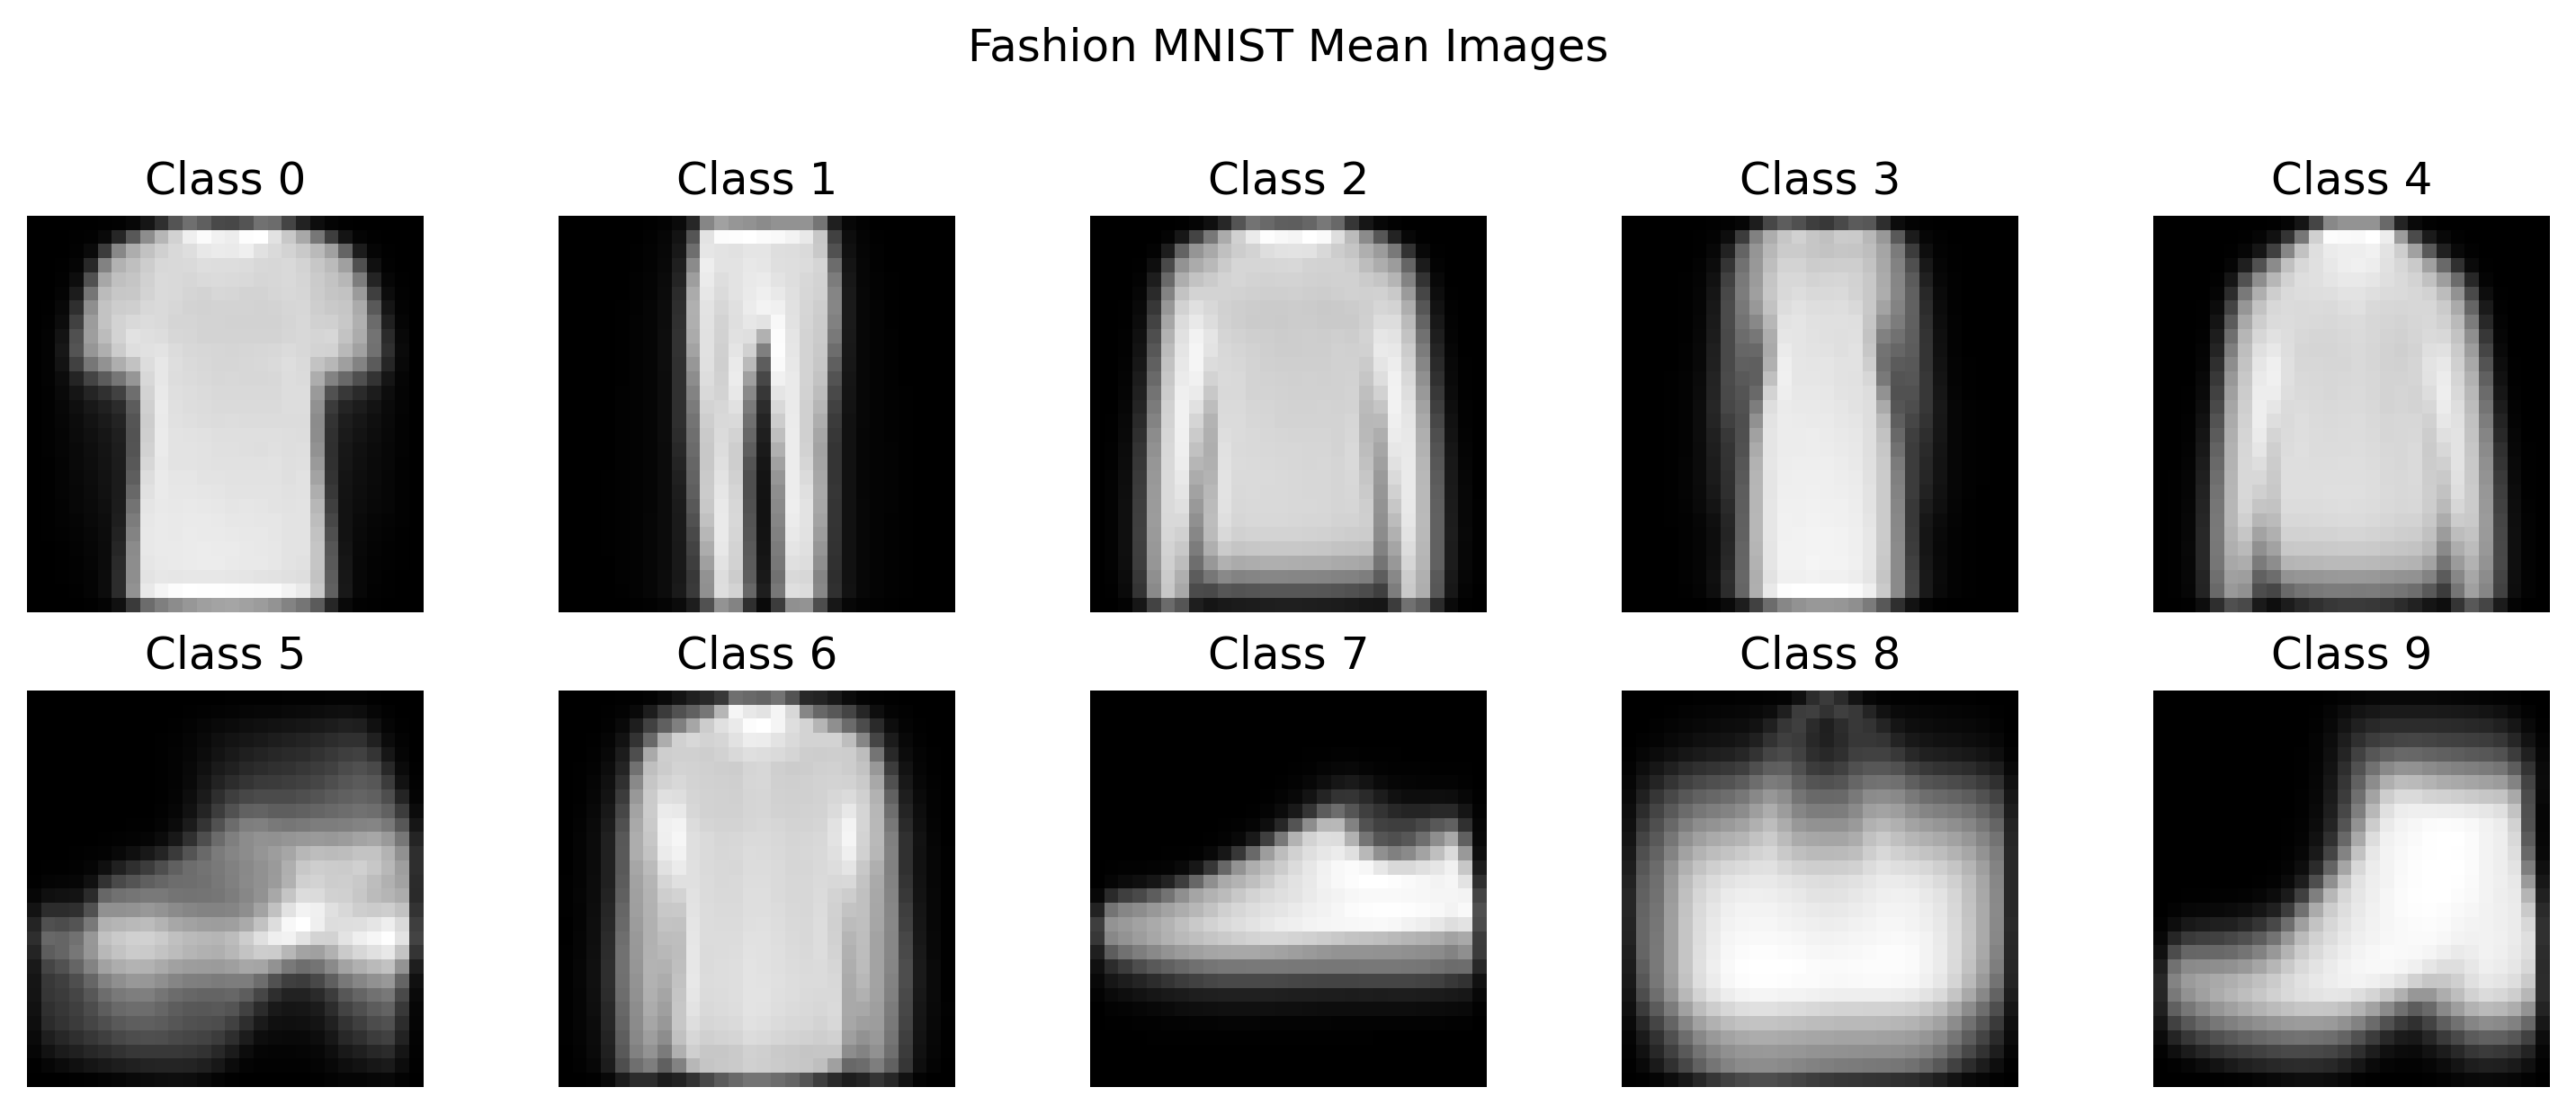
\includegraphics[width=0.9\linewidth]{mean_fashion.png}
    \caption{Ảnh trung bình theo lớp của Fashion MNIST.}
    \label{fig:mean-fashion}
\end{figure}

\begin{figure}[H]
    \centering
    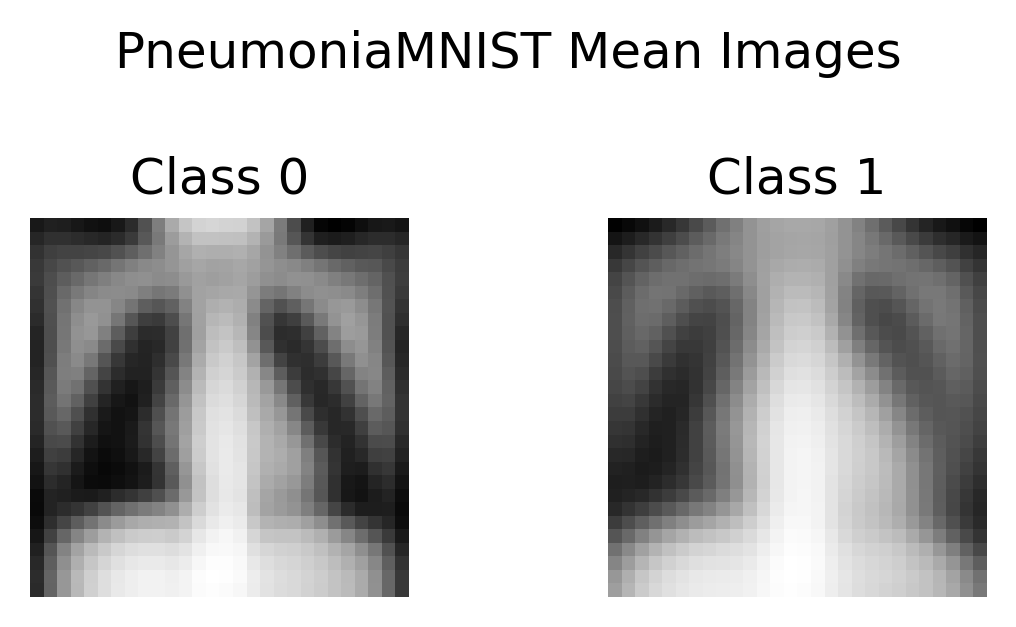
\includegraphics[width=0.6\linewidth]{mean_pneumonia.png}
    \caption{Ảnh trung bình của Normal và Pneumonia.}
    \label{fig:mean-pneumonia}
\end{figure}

\begin{figure}[H]
    \centering
    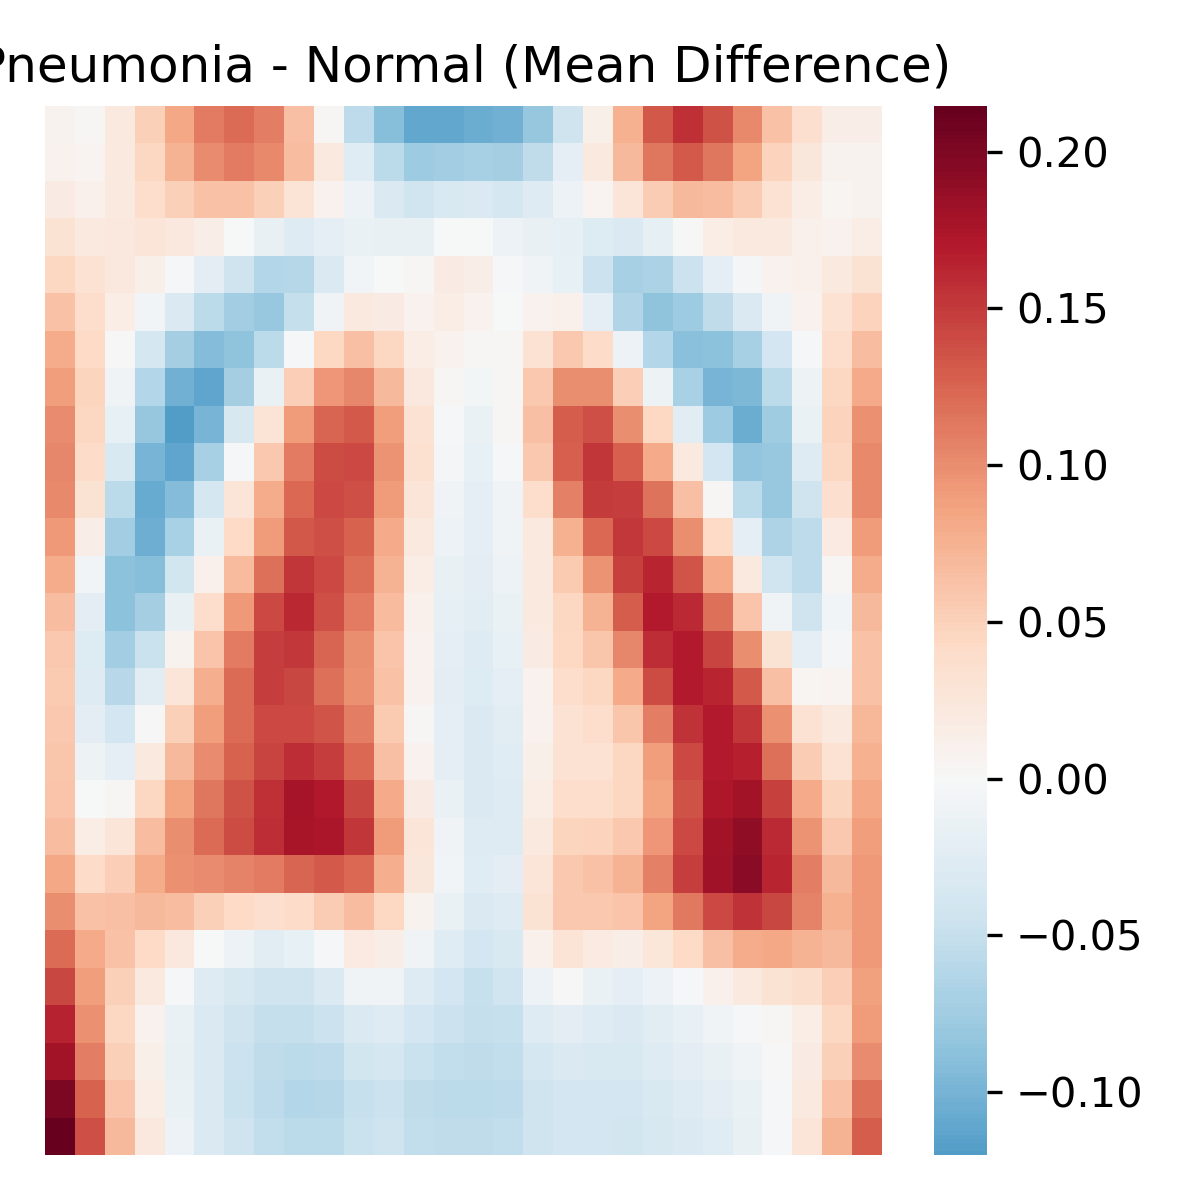
\includegraphics[width=0.55\linewidth]{pneumonia_difference_heatmap.png}
    \caption{Heatmap chênh lệch ảnh trung bình (PneumoniaMNIST: Pneumonia - Normal).}
    \label{fig:pneumonia-diff}
\end{figure}

\section{Phân tích Đặc trưng Thị giác}
\subsection{A. Cạnh biên (Canny Edge Detection)}
\subsubsection*{Mục tiêu}
Đối chiếu cấu trúc hình dạng giữa Fashion MNIST và PneumoniaMNIST thông qua bản đồ biên, nhằm quan sát mức độ rõ ràng của đường biên vật thể.

Về mặt nguyên lý, Canny tìm biên bằng cách làm trơn ảnh, tính độ lớn gradient $|\nabla I|$ và giữ lại các điểm có biên mạnh sau khi áp dụng ngưỡng kép (hysteresis). Một cách diễn đạt gọn là giữ lại các điểm thỏa $|\nabla I| \ge T_{high}$, và mở rộng qua các điểm lân cận có $T_{low} \le |\nabla I| < T_{high}$.

\subsubsection*{Thao tác}
Chọn ngẫu nhiên 5 ảnh Digit, 5 ảnh Fashion và 5 ảnh Pneumonia, áp dụng thuật toán \texttt{cv2.Canny()} để trích xuất viền\footnote{\url{https://en.wikipedia.org/wiki/Canny_edge_detector}}. Vẽ lưới 2x15: hàng trên là ảnh gốc, hàng dưới là ảnh biên tương ứng. Các ví dụ mang tính minh họa định tính, giúp so sánh cấu trúc biên giữa các miền dữ liệu.

\subsubsection*{Insight}
Digit MNIST thể hiện biên sắc nét và gọn, phù hợp với cấu trúc nét viết. Fashion MNIST tạo biên gọn và liên tục, phản ánh hình dạng vật thể rõ rệt. PneumoniaMNIST cho biên nhiễu và phân tán do cấu trúc giải phẫu (xương sườn, mô mềm), hàm ý bài toán y khoa dựa nhiều hơn vào \textit{texture} so với \textit{shape} (Hình~\ref{fig:canny-comparison}).

\begin{figure}[H]
    \centering
    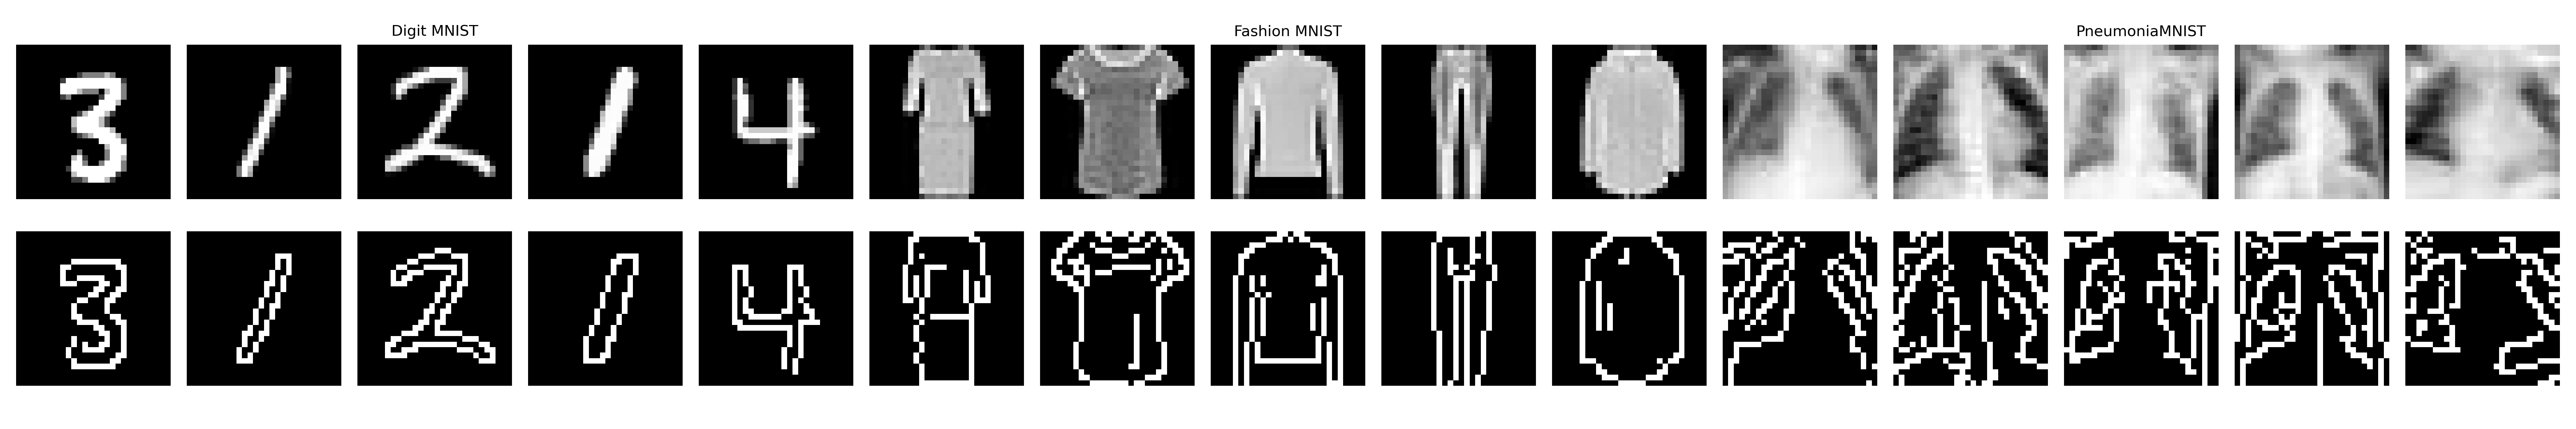
\includegraphics[width=0.95\linewidth]{canny_fashion_pneumonia.png}
    \caption{So sánh biên Canny giữa Digit MNIST, Fashion MNIST và PneumoniaMNIST.}
    \label{fig:canny-comparison}
\end{figure}

\subsection{B. Trích xuất đặc trưng thị giác truyền thống (CV Feature Extraction)}
\subsubsection*{Mục tiêu}
Chứng minh sự khác biệt về bản chất tín hiệu giữa ba miền dữ liệu thông qua các đặc trưng thị giác kinh điển: gradient, keypoints và texture.

Các kỹ thuật đều nhằm tóm tắt thông tin thị giác ở dạng vector đặc trưng: HOG đếm histogram hướng gradient theo ô lưới, còn GLCM thống kê tần suất đồng xuất hiện của cặp mức xám để suy ra texture.

\subsubsection*{Thao tác}
\textbf{HOG:} Chọn một ảnh ngẫu nhiên từ mỗi tập, áp dụng \texttt{skimage.feature.hog} (\textit{visualize=True}) và hiển thị cặp ảnh gốc - HOG.\footnote{\url{https://en.wikipedia.org/wiki/Histogram_of_oriented_gradients}}\\
\textbf{GLCM:} Với PneumoniaMNIST, tính \textit{Contrast} và \textit{Homogeneity} từ ma trận GLCM cho 200 ảnh Normal và 200 ảnh Pneumonia, sau đó vẽ boxplot so sánh.\footnote{\url{https://en.wikipedia.org/wiki/Co-occurrence_matrix}}

\subsubsection*{Insight}
HOG visualization cho thấy các cấu trúc gradient rõ ràng ở Digit MNIST và Fashion MNIST, phản ánh việc hai tập dữ liệu này phụ thuộc chủ yếu vào hình dạng và biên của vật thể. Ngược lại, ở PneumoniaMNIST, các đặc trưng HOG kém ổn định hơn, cho thấy thông tin phân biệt lớp nằm nhiều ở texture hơn là cấu trúc biên. Phân tích GLCM cũng cho thấy sự khác biệt texture giữa hai lớp: ảnh Normal có contrast cao hơn trong khi Pneumonia có homogeneity cao hơn, gợi ý rằng các đặc trưng texture có thể đóng vai trò quan trọng trong việc phân biệt hai lớp.

\begin{figure}[H]
    \centering
    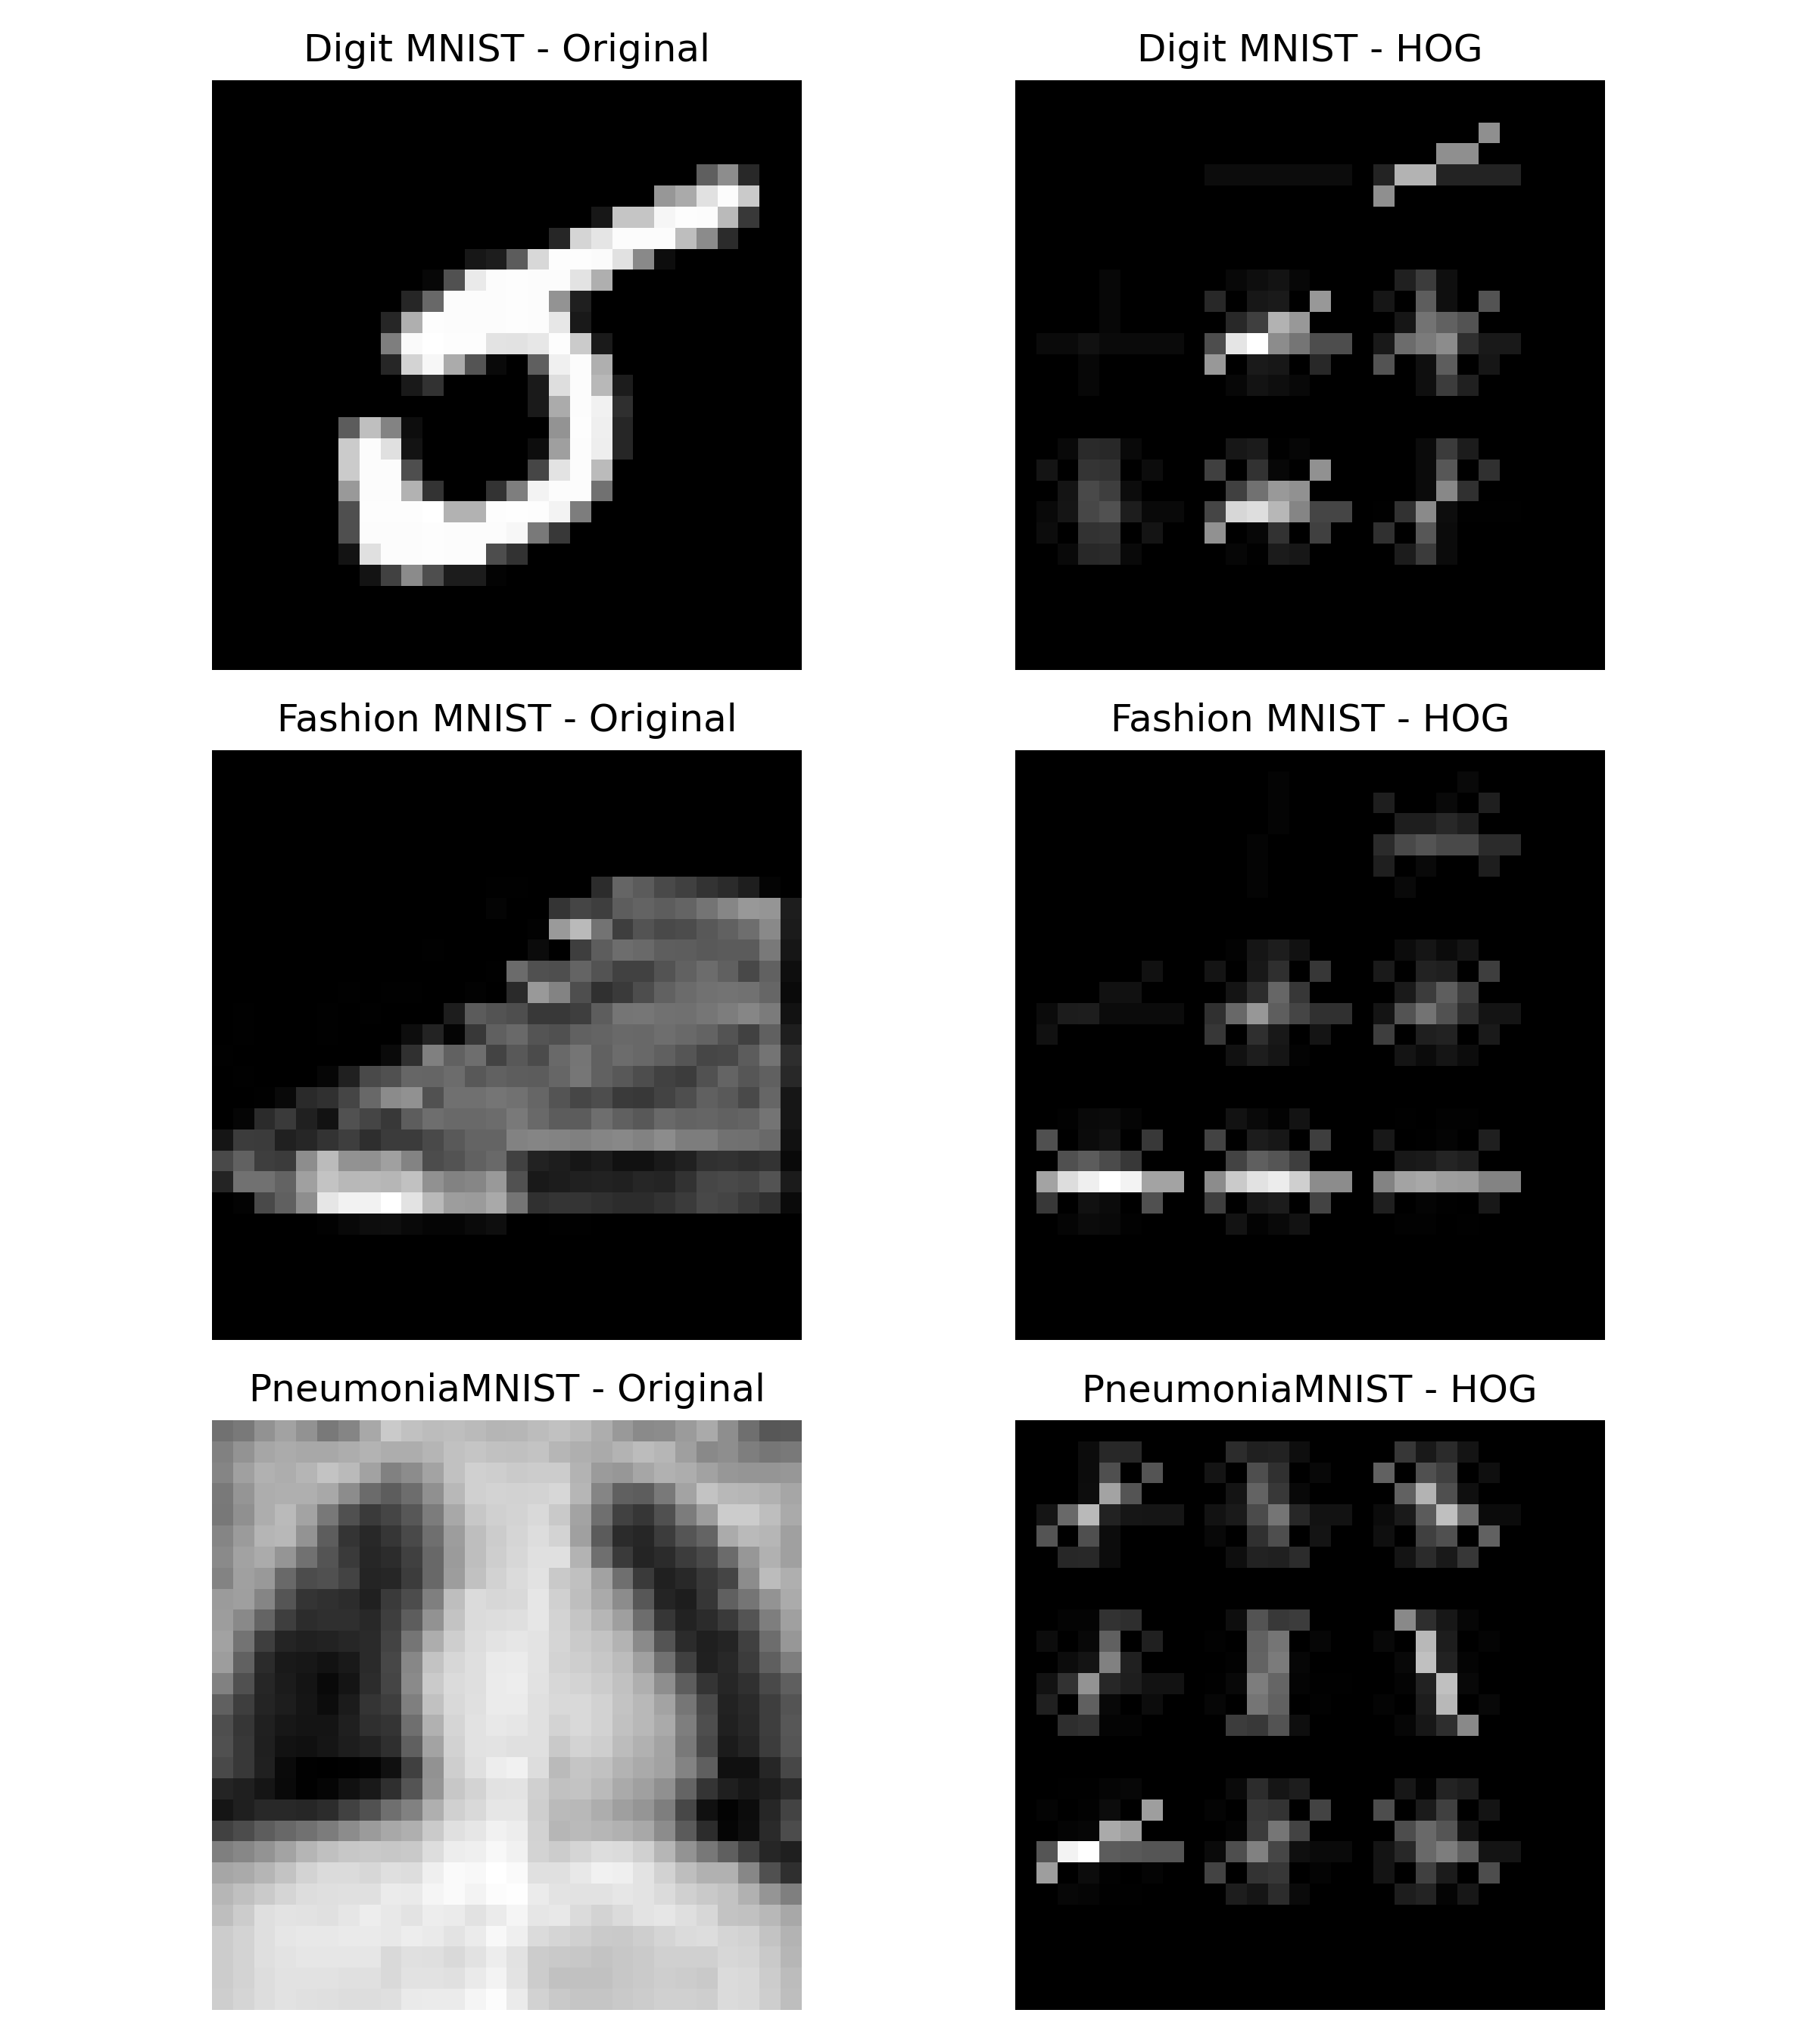
\includegraphics[width=0.85\linewidth]{hog_comparison.png}
    \caption{So sánh ảnh gốc và ảnh HOG cho mỗi tập dữ liệu.}
    \label{fig:hog-comparison}
\end{figure}

\begin{figure}[H]
    \centering
    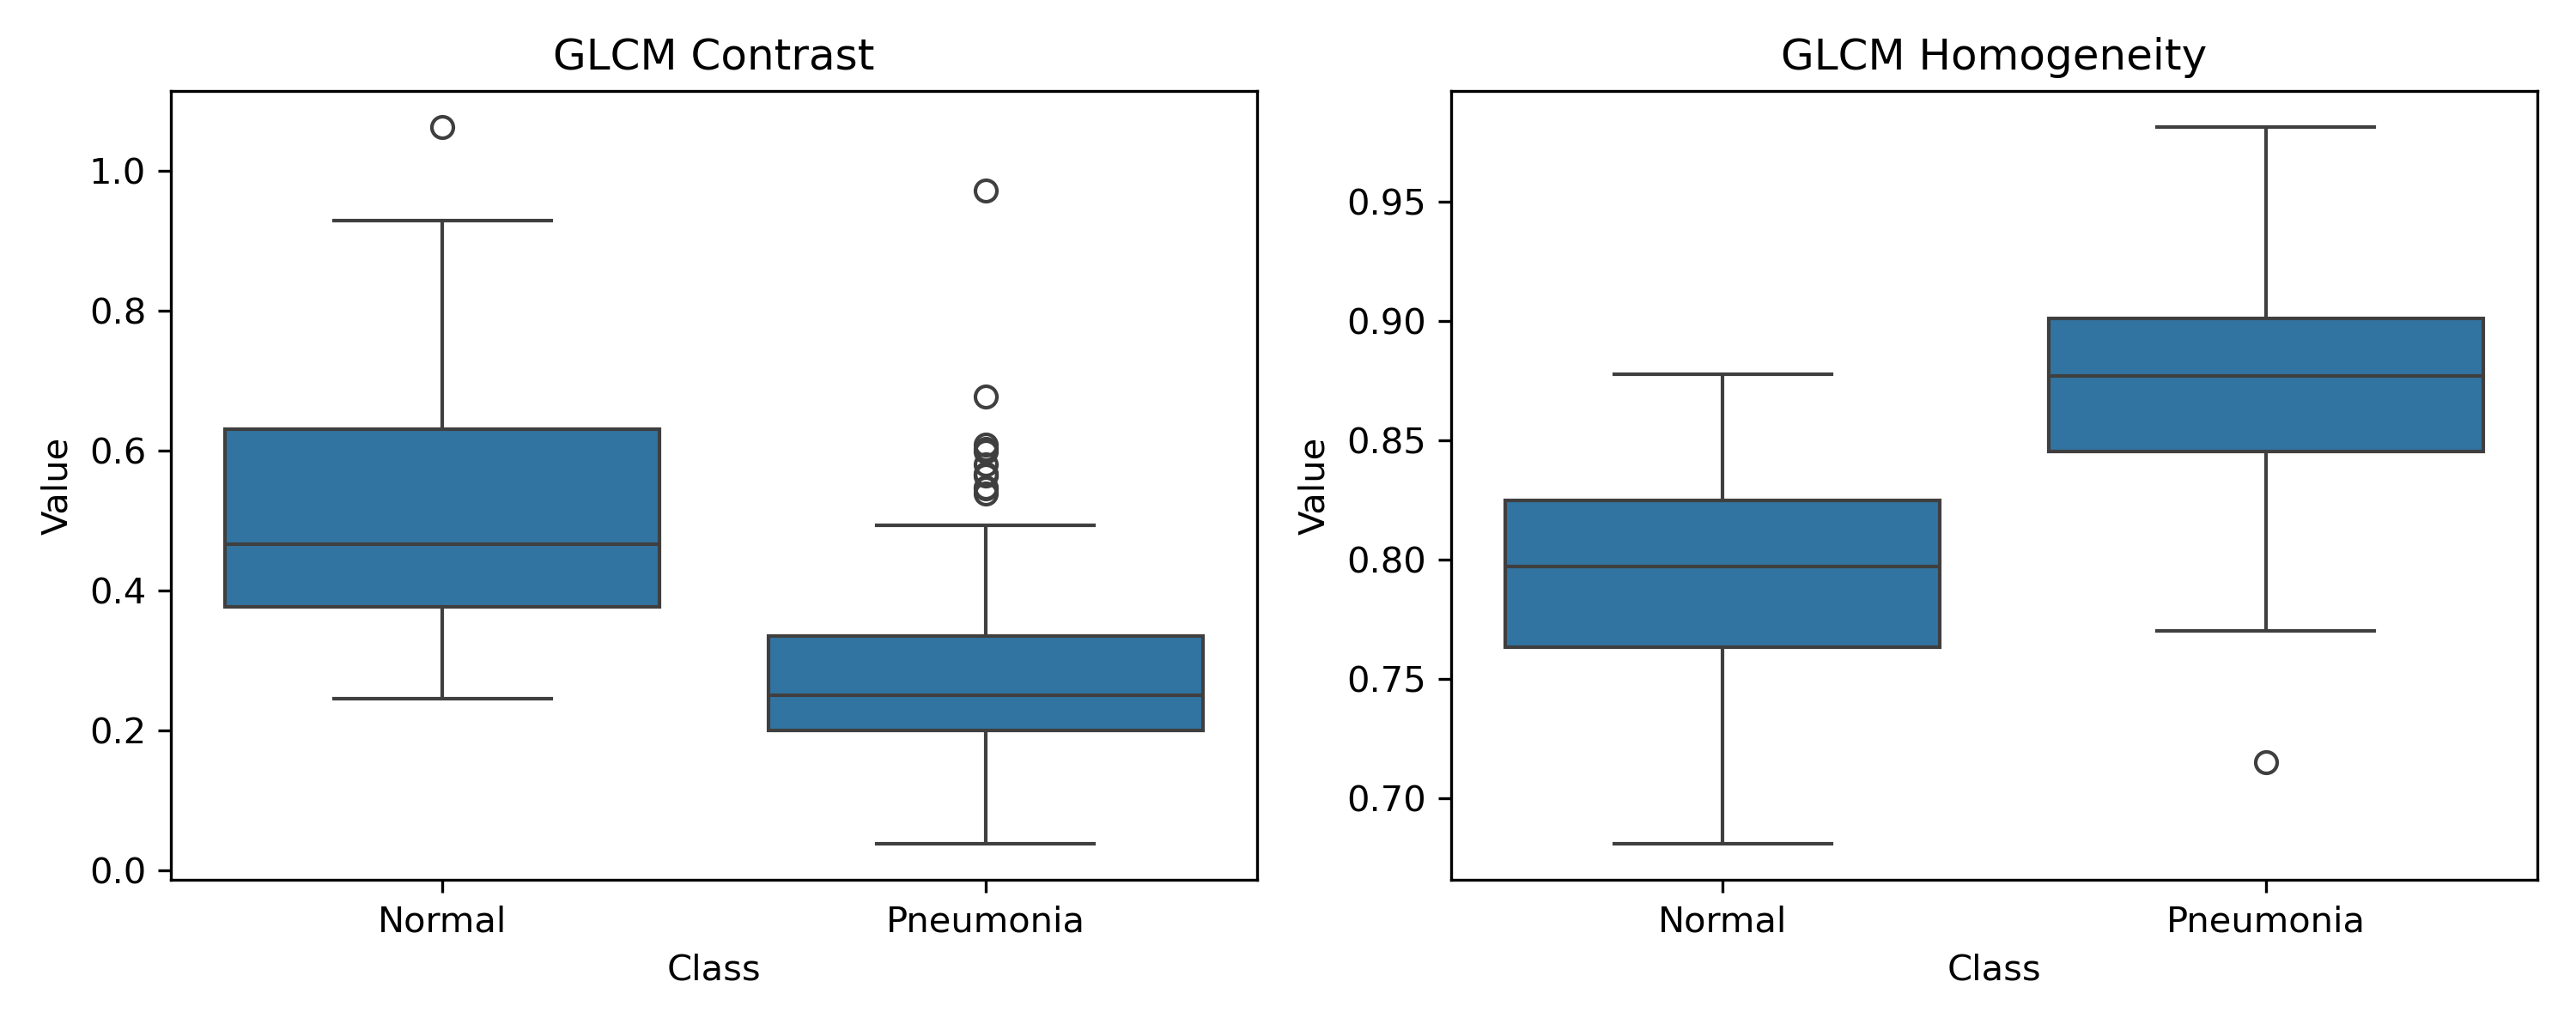
\includegraphics[width=0.85\linewidth]{glcm_boxplot.png}
    \caption{Boxplot so sánh đặc trưng GLCM (Contrast, Homogeneity) giữa Normal và Pneumonia.}
    \label{fig:glcm-boxplot}
\end{figure}

\section{Đánh giá Khả năng Phân tách (t-SNE)}
\subsection{Mục tiêu}
Đánh giá mức độ phân tách trong không gian đặc trưng giữa ba tập dữ liệu bằng t-SNE\footnote{\url{https://en.wikipedia.org/wiki/T-distributed_stochastic_neighbor_embedding}} và định lượng bằng điểm Silhouette.

t-SNE là phương pháp giảm chiều giúp trực quan hóa dữ liệu nhiều chiều bằng cách ánh xạ các điểm dữ liệu xuống không gian 2D, đồng thời cố gắng giữ cho các điểm giống nhau vẫn nằm gần nhau. Nhờ vậy, ta có thể quan sát trực quan cấu trúc cụm của dữ liệu và đánh giá khả năng phân tách giữa các lớp.

\subsection{Thao tác}
Làm phẳng ảnh thành vector 784 chiều, lấy mẫu ngẫu nhiên đúng 2000 ảnh cho mỗi tập, và chạy t-SNE với 2 thành phần. Trực quan hóa kết quả bằng scatter plot (1 hàng 3 cột). Tính Silhouette Score cho từng tập từ embedding t-SNE.\footnote{\url{https://en.wikipedia.org/wiki/Silhouette_(clustering)}} Việc giảm chiều dùng \texttt{sklearn.manifold.TSNE}, còn hệ số Silhouette tính bằng \texttt{sklearn.metrics.silhouette\_score}.

\subsection{Insight}
Nhìn trực quan vào biểu đồ t-SNE, Digit MNIST phân tách thành các cụm rải rác rõ rệt, trong khi PneumoniaMNIST hòa trộn thành một khối dữ liệu duy nhất (Hình~\ref{fig:tsne-comparison}). Tuy nhiên, cần lưu ý rằng Silhouette tính trên embedding t-SNE chỉ mang tính tham khảo vì t-SNE không bảo toàn khoảng cách toàn cục; do đó, các điểm số này nên được diễn giải thận trọng.

Trong đó dễ thấy, với tập Digit thì có sự chồng lấn nhiều giữa số 4 và 9 (thể hiện sự khó khăn trong sự phân biệt 2 lớp này). Còn với tập Fashion thì không còn là sự chồng chéo giữa 2 lớp, mà là nhiều lớp hơn (các vật thế có thể có nhiều hình dáng tương đồng nhau).

\textbf{Silhouette Score đạt được:}
\begin{itemize}
    \item \textbf{Digit MNIST:} 0.2018
    \item \textbf{Fashion MNIST:} 0.1776
    \item \textbf{Pneumonia MNIST:} 0.2357
\end{itemize}

\begin{figure}[H]
    \centering
    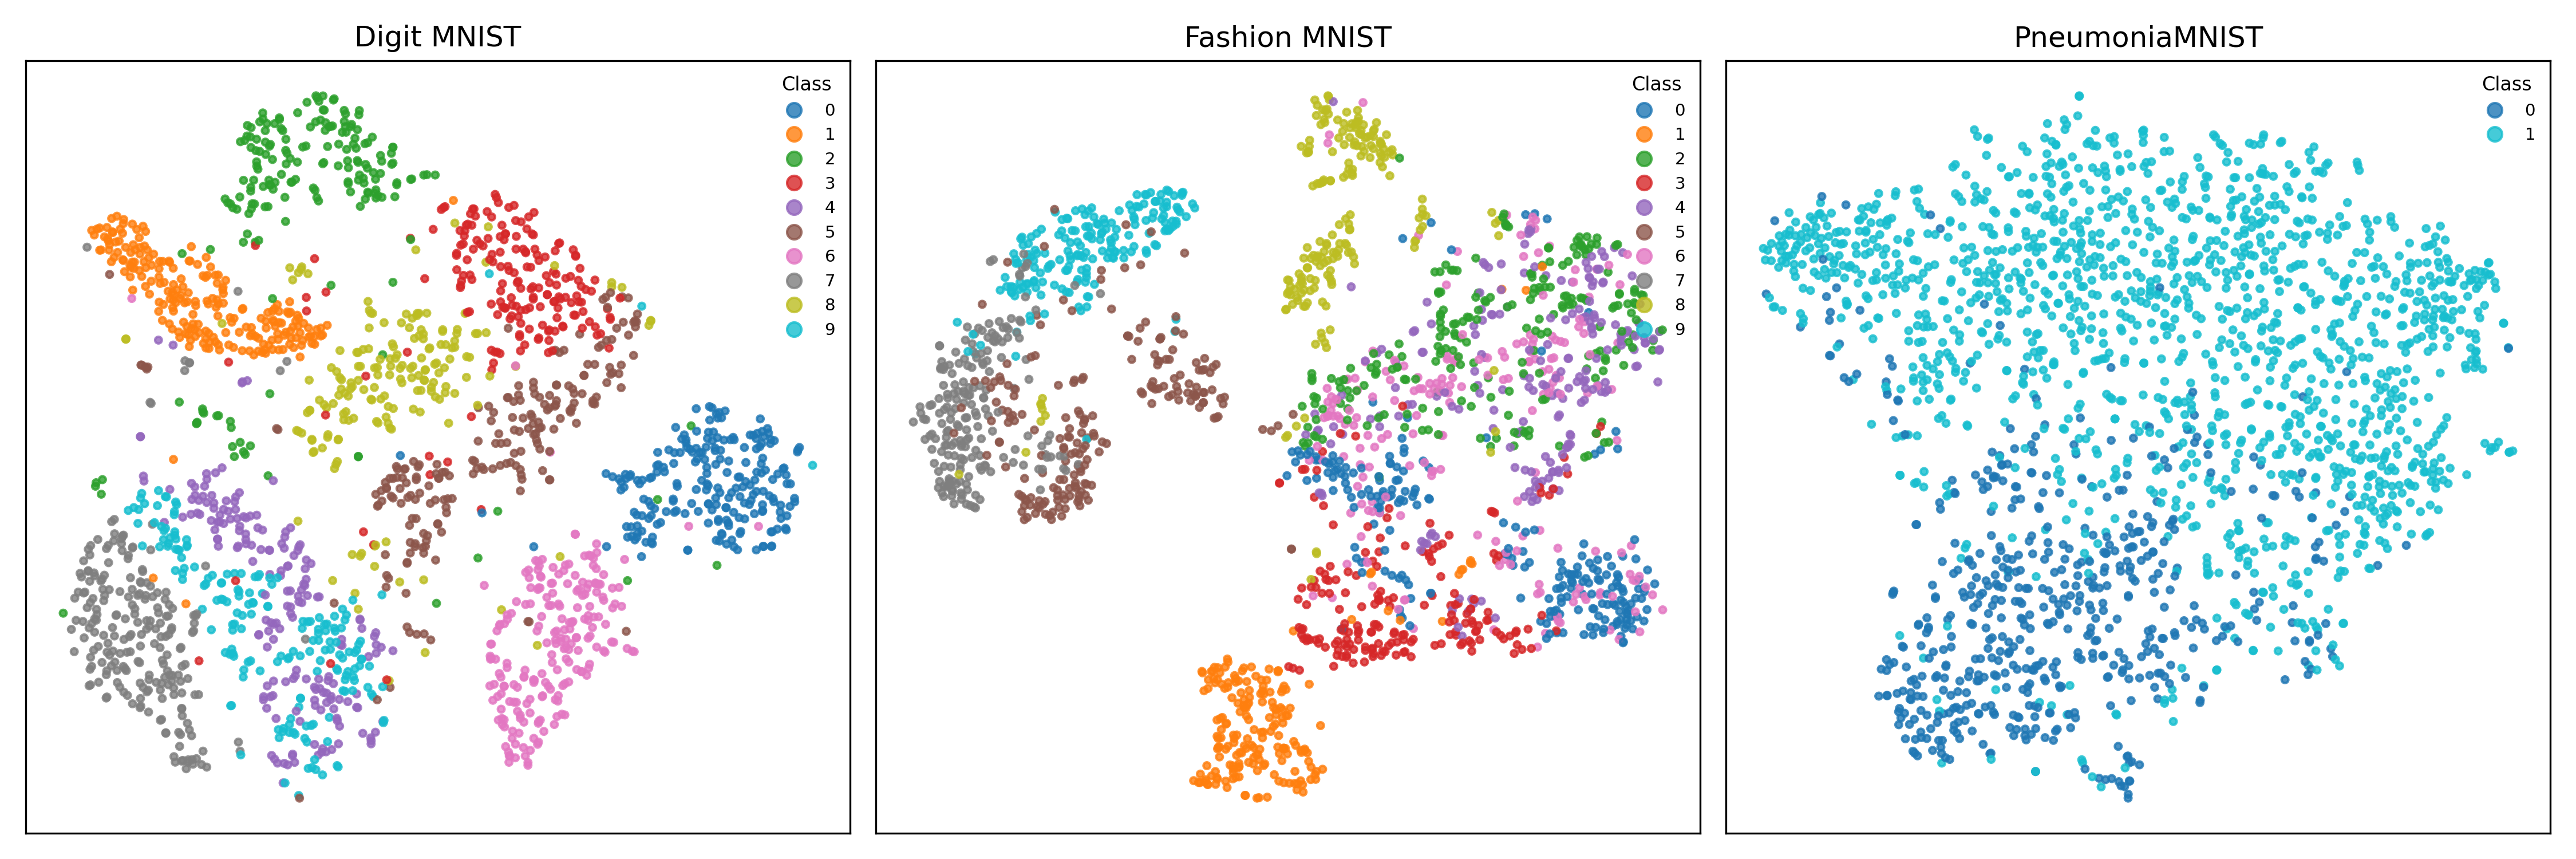
\includegraphics[width=0.9\linewidth]{tsne_comparison.png}
    \caption{So sánh t-SNE của Digit MNIST, Fashion MNIST và Pneumonia MNIST.}
    \label{fig:tsne-comparison}
\end{figure}

\section{Đo lường Độ Tương Đồng Cấu Trúc (SSIM)}
\subsection{Mục tiêu}
Định lượng mức độ tương đồng cấu trúc giữa các cặp ảnh X-quang để đánh giá mức độ khó của bài toán PneumoniaMNIST\footnote{\url{https://en.wikipedia.org/wiki/Structural_similarity}}.

SSIM đo mức độ giống nhau theo cấu trúc, với công thức chuẩn: $\mathrm{SSIM}(x,y)=\frac{(2\mu_x\mu_y + C_1)(2\sigma_{xy} + C_2)}{(\mu_x^2 + \mu_y^2 + C_1)(\sigma_x^2 + \sigma_y^2 + C_2)}$. Giá trị càng cao càng cho thấy hai ảnh có cấu trúc tương đồng.

\subsection{Thao tác}
Tính SSIM trung bình giữa 100 cặp Normal-Normal, 100 cặp Pneumonia-Pneumonia và 100 cặp Normal-Pneumonia. In kết quả ra màn hình và chèn vào báo cáo.

\subsection{Insight}
Ngay cả khi so sánh các ảnh trong cùng một lớp, SSIM của Normal-Normal chỉ đạt 0.5360 và Pneumonia-Pneumonia đạt 0.4361. Điều này phản ánh độ biến thiên (variance) rất cao trong dữ liệu y khoa do sự khác biệt về thể trạng bệnh nhân và điều kiện chụp X-quang. Đặc biệt, lớp Pneumonia có SSIM nội bộ thấp hơn hẳn, cho thấy các vùng tổn thương viêm phổi xuất hiện rất đa dạng và không đồng nhất về mặt cấu trúc.

Điểm SSIM chéo giữa Normal-Pneumonia giảm xuống mức thấp nhất là 0.3422. Điều này cho thấy cấu trúc toàn cục của hai lớp khác nhau, nhưng mức biến thiên nội bộ cao gợi ý rằng các đặc trưng toàn cục đơn giản có thể chưa đủ, và các phương pháp học đặc trưng (feature learning) có thể cần thiết để nắm bắt các tín hiệu tinh tế.

\textbf{SSIM trung bình thu được:}
\begin{itemize}
    \item \textbf{Normal-Normal:} 0.5360
    \item \textbf{Pneumonia-Pneumonia:} 0.4361
    \item \textbf{Normal-Pneumonia:} 0.3422
\end{itemize}

\section{Truy tìm Ngoại lai và Ảnh Hỏng}
\subsection{Mục tiêu}
Xác định các ảnh bất thường (quá tối hoặc quá sáng) trong PneumoniaMNIST nhằm mô phỏng rủi ro dữ liệu y khoa và đề xuất tiền xử lý.

Về mặt định lượng, z-score được tính theo $z = \frac{x - \mu}{\sigma}$, với $x$ là tổng cường độ điểm ảnh của một ảnh, $\mu$ là trung bình và $\sigma$ là độ lệch chuẩn của toàn bộ tập. Ảnh được xem là ngoại lai khi $|z| \ge 3$ (ngưỡng phổ biến cho ngoại lai cực trị).

\subsection{Thao tác}
Tính tổng cường độ pixel cho toàn bộ ảnh, sắp xếp và chọn 5 ảnh có tổng thấp nhất và 5 ảnh cao nhất. Tính \textit{z-score} cho mỗi ảnh để định lượng mức độ ngoại lai. Vẽ lưới 2x5 hiển thị các ảnh ngoại lai.

\subsection{Insight}
Xuất hiện các ảnh quá tối hoặc quá sáng cho thấy dữ liệu có vấn đề về phơi sáng (Hình~\ref{fig:pneumonia-outliers}). Điều này gợi ý cần cân bằng histogram (ví dụ CLAHE) hoặc chuẩn hóa độ tương phản ở giai đoạn huấn luyện.

\textbf{Z-score của các ảnh ngoại lai đại diện:}
\begin{itemize}
    \item \textbf{5 ảnh quá tối (Low intensity):} -4.08, -3.79, -3.72, -3.72, -3.65
    \item \textbf{5 ảnh quá sáng (High intensity):} 4.04, 3.14, 2.94, 2.80, 2.77
\end{itemize}

\begin{figure}[H]
    \centering
    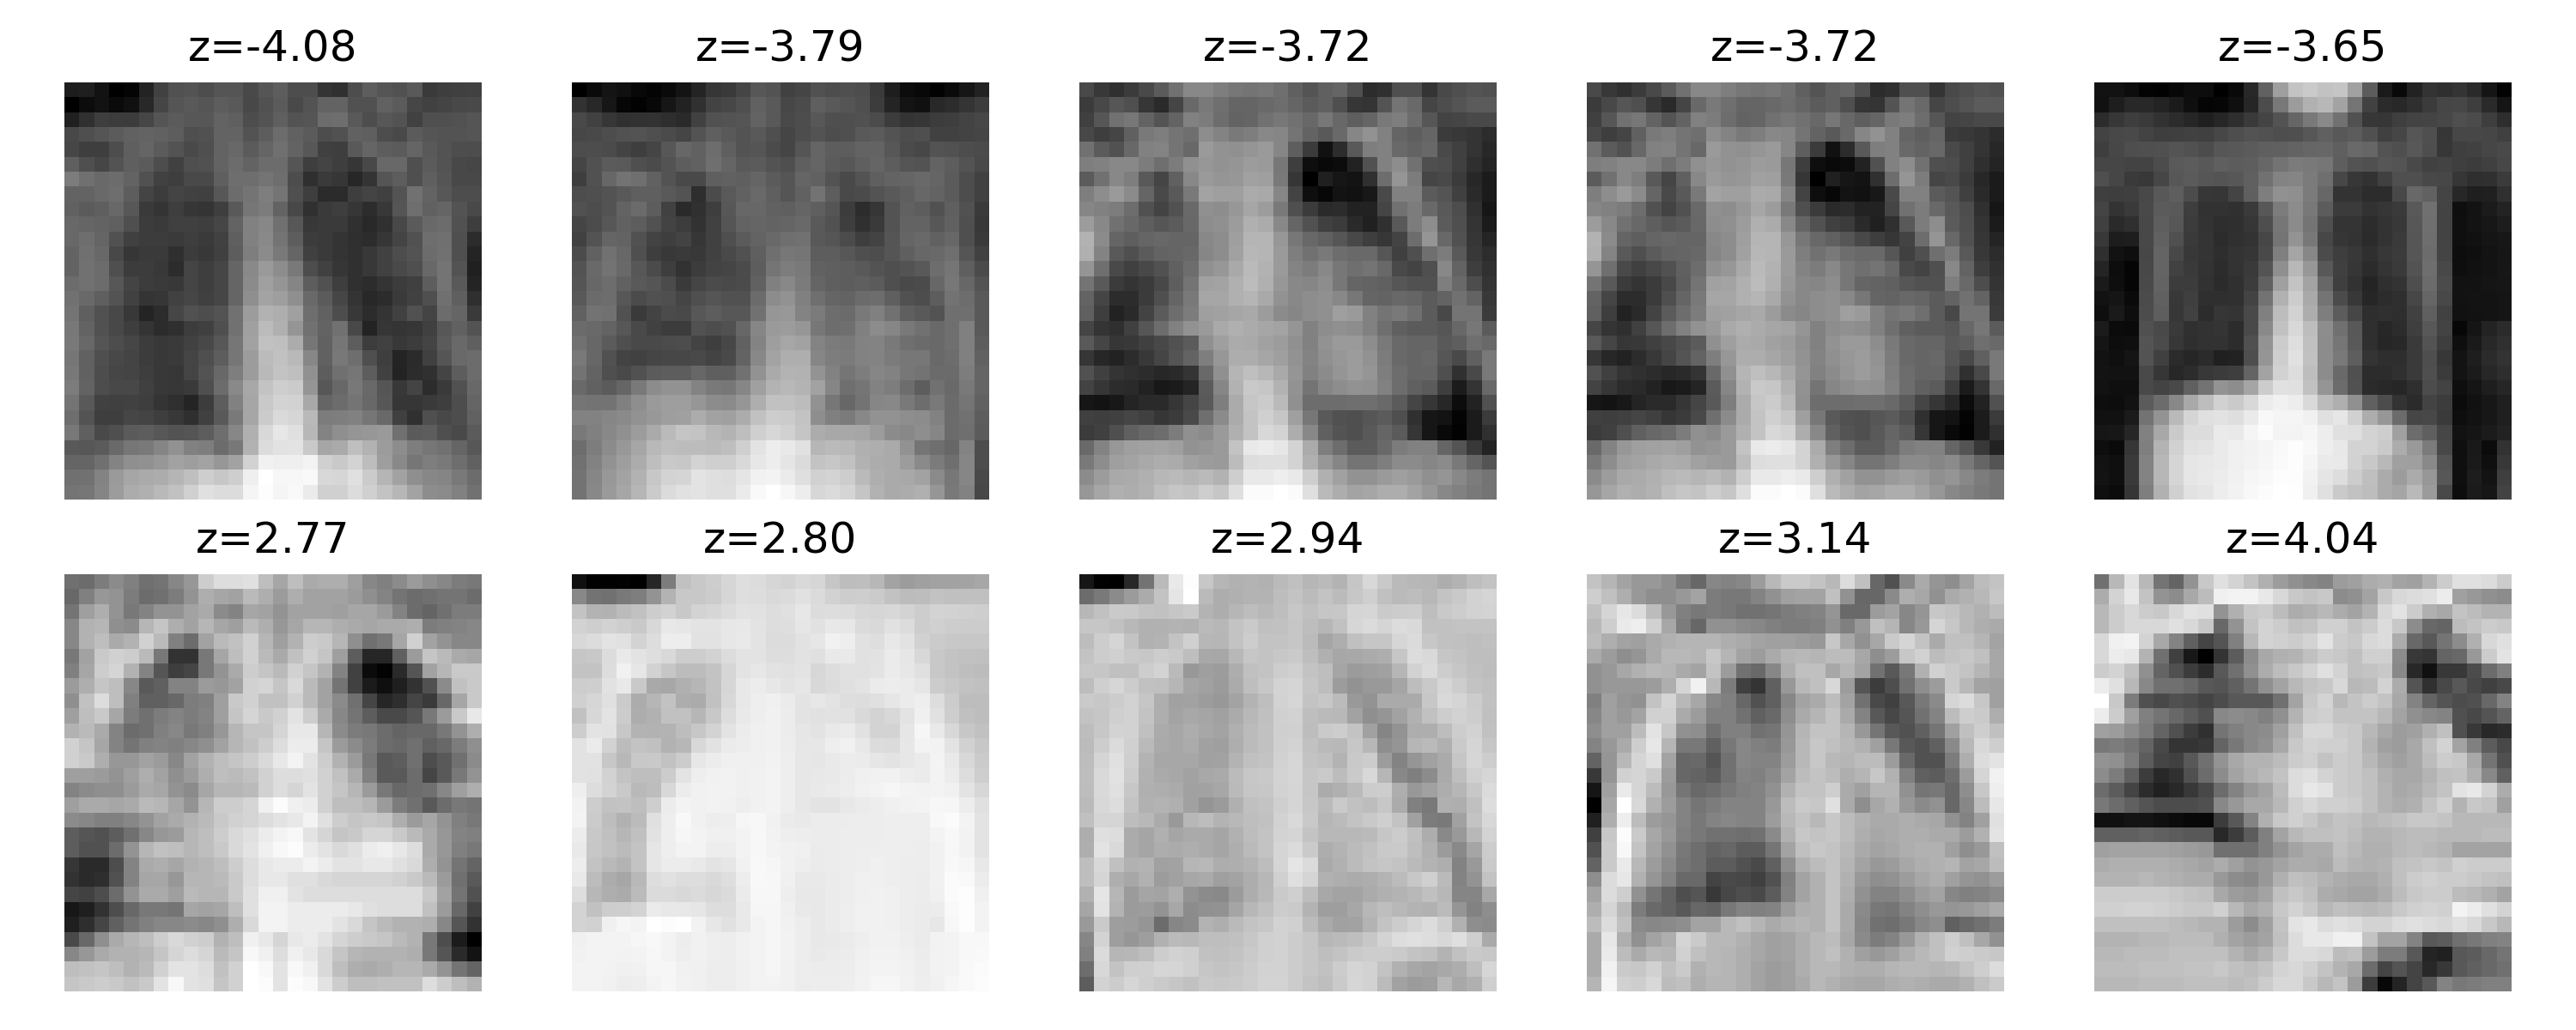
\includegraphics[width=0.8\linewidth]{pneumonia_outliers.png}
    \caption{10 ảnh ngoại lai (5 ảnh quá tối và 5 ảnh quá sáng) trong PneumoniaMNIST.}
    \label{fig:pneumonia-outliers}
\end{figure}


\end{document}